% Options for packages loaded elsewhere
\PassOptionsToPackage{unicode}{hyperref}
\PassOptionsToPackage{hyphens}{url}
%
\documentclass[
  11pt,
]{article}
\usepackage{amsmath,amssymb}
\usepackage{lmodern}
\usepackage{ifxetex,ifluatex}
\ifnum 0\ifxetex 1\fi\ifluatex 1\fi=0 % if pdftex
  \usepackage[T1]{fontenc}
  \usepackage[utf8]{inputenc}
  \usepackage{textcomp} % provide euro and other symbols
\else % if luatex or xetex
  \usepackage{unicode-math}
  \defaultfontfeatures{Scale=MatchLowercase}
  \defaultfontfeatures[\rmfamily]{Ligatures=TeX,Scale=1}
\fi
% Use upquote if available, for straight quotes in verbatim environments
\IfFileExists{upquote.sty}{\usepackage{upquote}}{}
\IfFileExists{microtype.sty}{% use microtype if available
  \usepackage[]{microtype}
  \UseMicrotypeSet[protrusion]{basicmath} % disable protrusion for tt fonts
}{}
\makeatletter
\@ifundefined{KOMAClassName}{% if non-KOMA class
  \IfFileExists{parskip.sty}{%
    \usepackage{parskip}
  }{% else
    \setlength{\parindent}{0pt}
    \setlength{\parskip}{6pt plus 2pt minus 1pt}}
}{% if KOMA class
  \KOMAoptions{parskip=half}}
\makeatother
\usepackage{xcolor}
\IfFileExists{xurl.sty}{\usepackage{xurl}}{} % add URL line breaks if available
\IfFileExists{bookmark.sty}{\usepackage{bookmark}}{\usepackage{hyperref}}
\hypersetup{
  pdftitle={Final Project for PS 531: A Pre-Analysis Plan},
  pdfauthor={Yea Jin Rha},
  hidelinks,
  pdfcreator={LaTeX via pandoc}}
\urlstyle{same} % disable monospaced font for URLs
\usepackage[left=1.25in,right=1.25in,top=1in,bottom=1in]{geometry}
\usepackage{color}
\usepackage{fancyvrb}
\newcommand{\VerbBar}{|}
\newcommand{\VERB}{\Verb[commandchars=\\\{\}]}
\DefineVerbatimEnvironment{Highlighting}{Verbatim}{commandchars=\\\{\}}
% Add ',fontsize=\small' for more characters per line
\usepackage{framed}
\definecolor{shadecolor}{RGB}{248,248,248}
\newenvironment{Shaded}{\begin{snugshade}}{\end{snugshade}}
\newcommand{\AlertTok}[1]{\textcolor[rgb]{0.94,0.16,0.16}{#1}}
\newcommand{\AnnotationTok}[1]{\textcolor[rgb]{0.56,0.35,0.01}{\textbf{\textit{#1}}}}
\newcommand{\AttributeTok}[1]{\textcolor[rgb]{0.77,0.63,0.00}{#1}}
\newcommand{\BaseNTok}[1]{\textcolor[rgb]{0.00,0.00,0.81}{#1}}
\newcommand{\BuiltInTok}[1]{#1}
\newcommand{\CharTok}[1]{\textcolor[rgb]{0.31,0.60,0.02}{#1}}
\newcommand{\CommentTok}[1]{\textcolor[rgb]{0.56,0.35,0.01}{\textit{#1}}}
\newcommand{\CommentVarTok}[1]{\textcolor[rgb]{0.56,0.35,0.01}{\textbf{\textit{#1}}}}
\newcommand{\ConstantTok}[1]{\textcolor[rgb]{0.00,0.00,0.00}{#1}}
\newcommand{\ControlFlowTok}[1]{\textcolor[rgb]{0.13,0.29,0.53}{\textbf{#1}}}
\newcommand{\DataTypeTok}[1]{\textcolor[rgb]{0.13,0.29,0.53}{#1}}
\newcommand{\DecValTok}[1]{\textcolor[rgb]{0.00,0.00,0.81}{#1}}
\newcommand{\DocumentationTok}[1]{\textcolor[rgb]{0.56,0.35,0.01}{\textbf{\textit{#1}}}}
\newcommand{\ErrorTok}[1]{\textcolor[rgb]{0.64,0.00,0.00}{\textbf{#1}}}
\newcommand{\ExtensionTok}[1]{#1}
\newcommand{\FloatTok}[1]{\textcolor[rgb]{0.00,0.00,0.81}{#1}}
\newcommand{\FunctionTok}[1]{\textcolor[rgb]{0.00,0.00,0.00}{#1}}
\newcommand{\ImportTok}[1]{#1}
\newcommand{\InformationTok}[1]{\textcolor[rgb]{0.56,0.35,0.01}{\textbf{\textit{#1}}}}
\newcommand{\KeywordTok}[1]{\textcolor[rgb]{0.13,0.29,0.53}{\textbf{#1}}}
\newcommand{\NormalTok}[1]{#1}
\newcommand{\OperatorTok}[1]{\textcolor[rgb]{0.81,0.36,0.00}{\textbf{#1}}}
\newcommand{\OtherTok}[1]{\textcolor[rgb]{0.56,0.35,0.01}{#1}}
\newcommand{\PreprocessorTok}[1]{\textcolor[rgb]{0.56,0.35,0.01}{\textit{#1}}}
\newcommand{\RegionMarkerTok}[1]{#1}
\newcommand{\SpecialCharTok}[1]{\textcolor[rgb]{0.00,0.00,0.00}{#1}}
\newcommand{\SpecialStringTok}[1]{\textcolor[rgb]{0.31,0.60,0.02}{#1}}
\newcommand{\StringTok}[1]{\textcolor[rgb]{0.31,0.60,0.02}{#1}}
\newcommand{\VariableTok}[1]{\textcolor[rgb]{0.00,0.00,0.00}{#1}}
\newcommand{\VerbatimStringTok}[1]{\textcolor[rgb]{0.31,0.60,0.02}{#1}}
\newcommand{\WarningTok}[1]{\textcolor[rgb]{0.56,0.35,0.01}{\textbf{\textit{#1}}}}
\usepackage{longtable,booktabs,array}
\usepackage{calc} % for calculating minipage widths
% Correct order of tables after \paragraph or \subparagraph
\usepackage{etoolbox}
\makeatletter
\patchcmd\longtable{\par}{\if@noskipsec\mbox{}\fi\par}{}{}
\makeatother
% Allow footnotes in longtable head/foot
\IfFileExists{footnotehyper.sty}{\usepackage{footnotehyper}}{\usepackage{footnote}}
\makesavenoteenv{longtable}
\usepackage{graphicx}
\makeatletter
\def\maxwidth{\ifdim\Gin@nat@width>\linewidth\linewidth\else\Gin@nat@width\fi}
\def\maxheight{\ifdim\Gin@nat@height>\textheight\textheight\else\Gin@nat@height\fi}
\makeatother
% Scale images if necessary, so that they will not overflow the page
% margins by default, and it is still possible to overwrite the defaults
% using explicit options in \includegraphics[width, height, ...]{}
\setkeys{Gin}{width=\maxwidth,height=\maxheight,keepaspectratio}
% Set default figure placement to htbp
\makeatletter
\def\fps@figure{htbp}
\makeatother
\setlength{\emergencystretch}{3em} % prevent overfull lines
\providecommand{\tightlist}{%
  \setlength{\itemsep}{0pt}\setlength{\parskip}{0pt}}
\setcounter{secnumdepth}{5}
\ifluatex
  \usepackage{selnolig}  % disable illegal ligatures
\fi
\usepackage[style=authoryear-comp,]{biblatex}
\addbibresource{finalbib.bib}

\title{Final Project for PS 531: A Pre-Analysis Plan}
\author{Yea Jin Rha}
\date{May 19, 2021}

\begin{document}
\maketitle

\begin{enumerate}
\def\labelenumi{\arabic{enumi}.}
\tightlist
\item
  Describe a substantive question in social science. What theory are you
  assessing? Why should anyone care? (2 paragraphs)
\end{enumerate}

~~~~~~My research question is `What is the effect of corruption
punishment information on corruption perceptions?' The theory that this
study aims to assess is the contingent self-commitment theory.
Originally,\textcite{levi_rule_1989} elaborated the concept of
contingent self-commitment and defined it as the contingent nature of a
commitment to comply with rules in a repeated setting without external
coercion. Later, \textcite{ostrom_governing_1990} used the concept in
her study to propose a potential solution for the `Tragedy of the
commons' problem. Tragedy of the commons is an economics problem in
which every individual has an incentive to consume a resource
(common-pool resource), but at the expense of every other
individual---with no way to exclude anyone from consuming. In the study,
Ostrom use the empirical evidence of long lasting common-pool resource
(CPR) situations and argues that the repeated games allow participants
to design their own contracts in light of the information they have at
hand. Essentially, the research emphasizes monitoring and graduated
sanctions as the crux information for citizen to develop contingent
self-commitment. \textcite{ostrom_governing_1990} claims that an
information of successful control would stimulate individual members to
engage in monitoring process which further consolidates the institution
of safeguarding public interest.\\
~\\
\hspace*{0.333em}\hspace*{0.333em}\hspace*{0.333em}\hspace*{0.333em}In
case of corruption, corruption free society which allows effective
governance is a common pool resource. A deviant action that harms public
interest for private gain is engaging in corruption. Corruption may be
viewed as a tragedy of the commons case because an individual has an
incentive to break corruption-free society by engaging in corruption at
the expense of every other citizen. If Ostrom's contingent
self-commitment is valid, a punishment information for corruption may
stimulate people to make self-commitment in controlling corruption which
may be reflected by the reduce corruption perceptions. Therefore,
theoretically, this paper is important for it examines the contingent
self-commitment theory. Moreover, previous
studies(\textcite{winters_lacking_2013};\textcite{boas_norms_2019}) use
corruption information which only informs who engaged in corruption in
their studies. Unlike the other studies, this research focus on the
corruption punishment information which substantively informs public how
well their society is functioning in protecting public interest. Thus,
this study may have empirical contribution as well by suggesting
potential solution for preventing corruption.

\begin{enumerate}
\def\labelenumi{\arabic{enumi}.}
\setcounter{enumi}{1}
\tightlist
\item
  The study you propose involves learning about a theory by observing
  certain of its implications. What one or two hypotheses that arise
  from the theory are you planning to assess? Why or how does the theory
  justify your expectations about these hypotheses? (1 or 2 paragraphs)
\end{enumerate}

~~~~~The study I propose involves learning about a contingent
self-commitment theory by observing of its implications. In this study,
I aim to test a hypothesis, a corruption punishment information reduces
corruption perceptions of the individuals. A contingent self-commitment
theory justifies my expectation about the hypothesis because it suggests
that a recognition of successful monitoring for unruly action, causing
harms to public interest, motivates people to self-engage in further
monitoring \textcite{ostrom_governing_1990}. Consequently, this leads
individuals to believe that their society is functioning well in
guarding public interest. Given the theory, it is plausible that an
information of punishment on corruption may motivate people to make
self-commitment in controlling corruption in their society. Further on,
such commitment would encourage individuals to perceive that the society
is less corrupt. Thus, this study examines the effect of corruption
punishment information on corruption perceptions of the individuals.
Also, grounding on the theory, I expect to observe the implication that
a punishment information would reduce corruption perceptions at an
individual level.

\begin{enumerate}
\def\labelenumi{\arabic{enumi}.}
\setcounter{enumi}{2}
\tightlist
\item
  What data and research design will help you answer this question? Why
  are you making these choices? (Remember that a statistical model is
  not a research design.) (2 paragraphs)
\end{enumerate}

~~~~My research question is `what is the effect of corruption punishment
information on corruption perceptions?' In order to answer the question
and to further obtain a causal inference, this research conducts a
survey experiment in South Korea from May 10th to May 18th in 2018.
(Although the data was collected in 2018, I did not run any statistical
analysis yet.) South Korea experienced the presidential corruption
scandal in 2016 and the constitutional court decided to impeach the
president in that year. Here, I assume that the fact, corruption
occurred, is still evident but the public's memory of exact court
sentences for each malefactor faded after two years. This would allow
the operation of treatment in the survey context either by reminding or
newly informing the corruption punishment information to the
participants. A corruption experience in South Korea makes it a good
case to examine the contingent self-commitment theory and to test my
hypothesis. This is because the corruption scandal was large in scale
that it involved incumbent president and the chief executive officer of
Korea's top business company, Samsung. More importantly, I was the first
time ever in South Korea that the legal accusation was clearly imposed
on the culprits for their malfeasance.\\
~\\
\hspace*{0.333em}\hspace*{0.333em}\hspace*{0.333em}\hspace*{0.333em}\hspace*{0.333em}In
terms of the treatment, the court decision for the punishment, is
randomly proposed to the participants through a vignette before they
answer the survey questions. Participants in the control group view a
vignette which only has the information that a grand scale corruption
occurred in Korea. Next, the survey question measures the potential
outcome, corruption perceptions, by asking `How frequently do you expect
the use of authority for private gain or personal connection will occur
in the future?' Respondents answer the degree of perceived corruption
for the future in five-level Likert Scale from `1' indicating definitely
more to `5' referring definitely less. The total number of 457 people
participated in the survey, and 229 were treated while the 228 were not
treated. The data collection process continued until it fulfills the
minimum number of 227 responses that fully answered the questions.
Overall, the survey experiment design compares the potential outcome of
the treated group and the control group and assess if there is an effect
of corruption punishment information on corruption perceptions.

\begin{enumerate}
\def\labelenumi{\arabic{enumi}.}
\setcounter{enumi}{3}
\tightlist
\item
  What are the advantages and disadvantages of this research design to
  addressing your question? (2 paragraphs discussing \textbf{both}
  advantages and disadvantages of the research design; could be 1
  paragraph for advantages and 1 for disadvantages or combined
  discussion across 2 paragraphs.)
\end{enumerate}

~~~~~~The design of survey experiment has two major advantages in
addressing my question. First, survey experiment induces less bias than
direct questioning in measuring sensitive attitudes and perceptions.
(\textcite{blair_design_2015};\textcite{rosenfeld_empirical_2016};\textcite{lensvelt-mulders_meta-analysis_2005})
Since the outcome variable which the study intends to measure is
corruption perceptions, and it is a sensitive issue that respondents
often veil their thoughts, survey experiment may provide more valid
measurement of corruption than the other types of research designs.
Second, survey experiment measures causal relationships by randomly
assigning respondents to an experimental condition or a control group.
This overcomes the limitation of observational study which often draws
correlation instead of causal inference. Thus, in my study, survey
experiment is useful because it captures the potential effect of
corruption punishment information and the casual inference by
randomizing the treatment assignment process.\\
\hspace*{0.333em}\hspace*{0.333em}\hspace*{0.333em}\hspace*{0.333em}\hspace*{0.333em}\hspace*{0.333em}On
the contrary, there are important limitations in using survey
experiment. First, a survey experiment may capture the explicit attitude
which a respondent is aware of, whereas it would not measure the
implicit attitude which is not recognized by the respondent oneself
(\textcite{nosek_implicitexplicit_2007}). Also, the possibility of
contamination in the process of survey experiment such as, question
ordering effect and unidentical interpretation of the terms in the
question by the respondents exist. Such limitations may reduce the
validity of the measured perceptions of corruption in this study.
Second, survey experiment may involve confounding, information
equivalence problem, and pre-treatment contamination which may result in
bias regarding causal inference
(\textcite{diaz_survey_2020};\textcite{dafoe_information_2018}). Because
survey experiment is less conservative in a way to observe
counterfactual cases than hard science experiment, the causal inference
that a researcher draw may not be valid. This requires a scholar to be
cautious about the possible bias in survey experiment, and thus, need to
be careful in interpreting the result. Such difficulty applies to this
research as well. Unidentified confounding variables, unidentical
interpretation of the question and the pre-treatment effect outside of
the survey context may interrupt accurate observation of the causal
relationship between corruption punishment information and corruption
perceptions.

\begin{enumerate}
\def\labelenumi{\arabic{enumi}.}
\setcounter{enumi}{4}
\tightlist
\item
  Describe your measures and any indices you construct. (1 paragraph)
\end{enumerate}

~~~~In terms of the outcome variable the survey question that asks, `How
frequently do you expect the use of authority for private gain or
personal connection will occur in the future?' measures corruption
perceptions. The responses ranges within the five-level Likert Scale
from `1' indicating definitely more to `5' referring definitely less.
Hence, higher the number, survey participant believe society would be
less corrupt in in the future. When it comes to the explanatory
variable, the treatment is the stimulus in the survey which is a
detailed written information how each accused culprit ended up with
final legal sentences, or punishments.

\begin{enumerate}
\def\labelenumi{\arabic{enumi}.}
\setcounter{enumi}{5}
\item
  Use data to make the case that your research design allows you to
  interpret observed quantities (like observed data comparisons or
  parameters of models fit to data) as theoretically relevant and clear:
  (Most people will only have to do either 6.1 and 6.2 \textbf{or} 6.3
  and 6.4 here depending on whether you have a randomized design or an
  observational design).

  \begin{enumerate}
  \def\labelenumii{\roman{enumii}.}
  \tightlist
  \item
    \textbf{If you are using an randomized study design}, explain how
    the experiment will help you make the case for interpretable
    comparisons. What counter arguments and/or weaknesses of your
    approach might you expect? (For example, how will you think about
    Hawthorne effects or alternative explanations of your results
    arising from crticisms of your measurement and conceptualization
    strategy or missing data problems.) (1 paragraph)
  \end{enumerate}
\end{enumerate}

~~~~The survey experiment will help me make the case for interpretable
comparisons by randomly assigning treatment, the stimulus information of
corruption punishment, to the survey participants. This way, we can
compare the outcome of the treated group and the control group in order
to measure the effect of the treatment and to make causal implication.
In this randomized study design, potential counter argument exists. One
might argue that experimental setting may modify respondents' behavior
causing Hawthorne effect and interrupt the measurement process. A
possible leeway in this study is that the experiment was an online
survey and collected the responses anonymously. Some others might argue
that the treatment in the survey experiment setting does not actually
measures the effect of corruption punishment information but the framing
effect of the survey. This criticism is valid because it is true that
social scientists cannot infuse manipulated information to the
participants of an experiment for ethical reasons. Nevertheless,
randomization is difficult under an observational study and thus,
scholars intend to approach, as if experiment setting, for achieving
causal inference through randomization process in exchange of less
accurate and valid measurement. Still others may concern the missing
data problem in the study. However, there will be no missingness in
treatment in this experimental setting and the collected dataset
indicates no missingness in the outcome variable as well. Ultimately,
survey experiment is not a panacea to make a causal inference nor allows
perfect measurement of the treatment effect. Therefore, I should be
careful in interpreting the result of survey experiment and be aware of
the potential biasness in testing the hypothesis.

\begin{enumerate}
\def\labelenumi{\roman{enumi}.}
\setcounter{enumi}{1}
\tightlist
\item
  \textbf{If you are using a randomized study design}, explain how you
  will know that your randomization and/or other aspects of your design
  turned out as they should (for example, you might explain about
  randomization tests here). (1 paragraph)
\end{enumerate}

~~~~I will know that my randomization turned out as it should be by
checking the balance of treatment and control group of the survey
experiment using a statistical tool, `Xbalance'. Xbalance tests
conditional independence of the treatment variable and the covariates
within strata by calculating standardized mean differences along each
covariate with and without the stratification. (see detailed information
on
\url{https://www.rdocumentation.org/packages/RItools/versions/0.1-17/topics/xBalance})
The result of xbalance shows that \(p\)-value (0.878) is greater than
0.05. This indicates that there is not enough evidence to support the
difference in background variables of the treated and control group.

\% latex table generated in R 4.0.5 by xtable 1.8-4 package \% Wed May
19 02:21:11 2021

\begin{table}[ht]
\centering
\begin{tabular}{lrrrrrrr}
  \hline
 & treatment=0 & treatment=1 & adj.diff & adj.diff.null.sd & std.diff & z &  \\ 
  \hline
sex & 1.50 & 1.51 & 0.01 & 0.05 & 0.01 & 0.14 &     \\ 
  age\_quart & 3.54 & 3.52 & -0.02 & 0.16 & -0.01 & -0.12 &     \\ 
  residence & 5.90 & 5.54 & -0.37 & 0.39 & -0.09 & -0.94 &     \\ 
  party\_affiliation & 3.93 & 3.94 & 0.01 & 0.26 & 0.00 & 0.05 &     \\ 
  pol\_ideo & 2.75 & 2.78 & 0.03 & 0.08 & 0.03 & 0.34 &     \\ 
  edu & 3.15 & 3.20 & 0.05 & 0.11 & 0.04 & 0.47 &     \\ 
  income & 3.83 & 3.60 & -0.23 & 0.21 & -0.10 & -1.11 &     \\ 
   \hline
\end{tabular}
\end{table}

\begin{enumerate}
\def\labelenumi{\arabic{enumi}.}
\setcounter{enumi}{6}
\tightlist
\item
  Explain your plans for any missing data or extreme outcome or
  covariate values you may encounter when you get the real data (or
  perhaps you have the background data but not the real outcomes, so you
  can explain your plans for such data issues in that case here too). (1
  or 2 paragraphs)
\end{enumerate}

~~~~~~Missingness in data may happen regarding outcome, treatment and
covariate variables, respectively. First, the collected dataset
indicates that there are no missing values in both outcome and treatment
variable. Also, missingness in covariates is not a critical issue in
this study because it only focuses on the effect of the treatment on the
outcome variable. The expected structural model in this paper does not
consider the background variables. Next, it is unlikely that the data
would have an extreme outcome value because the survey response ranges
from 1 to 5 measured in ordinal scale.

\begin{enumerate}
\def\labelenumi{\arabic{enumi}.}
\setcounter{enumi}{7}
\tightlist
\item
  What statistical tests do you plan to use? Explain why you chose these
  tests and any decision making criteria you will use upon seeing the
  results of the tests. You should also engage with the problem of
  multiple testing here if you are going to show the results of more
  than one test. (Recall that confidence intervals and hypothesis tests
  convey more or less the same information. So a confidence interval is
  a form of testing.) (1 paragraph)
\end{enumerate}

~~~~~~I am going to use robust linear regression to test my hypothesis.
There are two major reasons for using this statistical test. First, this
research is interested in finding a causal inference of corruption
punishment information on corruption perceptions. Mainly, the study aims
to examine the effect of punishment information on the potential
outcome. The permutation testing involved in the linear regression
suggest how much evidence the research design provide about a causal
claim. Therefore, in testing the hypothesis, I examine \(p\)-value using
robust linear regression analysis which describes the relationship
between the observed test statistic and the distribution of possible
hypotheses given null effect. Although the permutation testing does not
provide exact effect size of the treatment, it reflects if the observed
data we have provide sufficient evidence to reject the null hypothesis.
Second, robust linear regression allows us not to assume
homoskedasticity of the standard error which leads to over fitting
problem in terms of outlier or extreme and influential observations.
Although, robust linear regression model does not control for
covariates, it can increase the precision of the estimation. Thus, once
the distribution of the test statistics based on the central limit
theorem and the design with the heteroskedasticity-consistent standard
error is made, I will check the \(p\)-value and the confidence interval
to find out the probability of seeing the observed estimate more extreme
given that the null hypothesis is true. The following table refers to th
robust linear regression of corruption perceptions on treatment.

\% latex table generated in R 4.0.5 by xtable 1.8-4 package \% Wed May
19 02:21:11 2021

\begin{table}[ht]
\centering
\begin{tabular}{rrrrrrrr}
  \hline
 & Estimate & Std. Error & t value & Pr($>$$|$t$|$) & CI Lower & CI Upper & DF \\ 
  \hline
(Intercept) & 3.04 & 0.10 & 31.79 & 0.00 & 2.85 & 3.22 & 455.00 \\ 
  treatment & -0.08 & 0.13 & -0.59 & 0.55 & -0.34 & 0.18 & 455.00 \\ 
   \hline
\end{tabular}
\label{tab:lm_robust Regression}
\end{table}

\begin{enumerate}
\def\labelenumi{\arabic{enumi}.}
\setcounter{enumi}{8}
\tightlist
\item
  Explain how you will judge the performance of those tests. Will you
  only use simple false positive rate and power? Or do you need to add
  family-wise error rate? false discovery rate? Or something else?
  Explain why you made this choice. (1 paragraph)
\end{enumerate}

~~~~I will judge the performance of the tests by simulating the design.
Because I am testing a single hypothesis the adjustment to control the
error rates is not required. Also, family-wise error rate and false
discovery rate that needs to be considered in multiple hypothesis
testing is not necessary in this study. To be more specific, I intend to
run a simulation and calculate the probability of rejecting a null
hypothesis when the true effects are 0 (false positive rate). A good
test should have low false positive error rate. In other words, the
proportion of small \(p\)-values should be no larger than \(alpha\)
(level of the test). Also, through the simulation, this paper will
calculate the power of the test which indicates the probability to
detect the effect when the true effect is not 0. In terms of power, a
good hypothesis test should have high statistical power.

\begin{enumerate}
\def\labelenumi{\arabic{enumi}.}
\setcounter{enumi}{9}
\tightlist
\item
  Show and explain how your test performs in regards those properties
  (at least you will show false positive rate and power). (2--4
  paragraphs)
\end{enumerate}

\begin{Shaded}
\begin{Highlighting}[]
\NormalTok{myvarest }\OtherTok{\textless{}{-}} \ControlFlowTok{function}\NormalTok{(data)\{}
\NormalTok{variance\_diff }\OtherTok{\textless{}{-}} \FunctionTok{with}\NormalTok{(data,}\FunctionTok{var}\NormalTok{(Y[Z}\SpecialCharTok{==}\DecValTok{1}\NormalTok{]) }\SpecialCharTok{{-}} \FunctionTok{var}\NormalTok{(Y[Z}\SpecialCharTok{==}\DecValTok{0}\NormalTok{]))}
\NormalTok{df }\OtherTok{\textless{}{-}} \FunctionTok{data.frame}\NormalTok{(}\AttributeTok{estimate=}\NormalTok{variance\_diff)}
\FunctionTok{return}\NormalTok{(df)}
\NormalTok{\}  }

\NormalTok{design }\OtherTok{\textless{}{-}}
  \FunctionTok{declare\_model}\NormalTok{(}\AttributeTok{data =}\NormalTok{ pap) }\SpecialCharTok{+}
  \FunctionTok{declare\_potential\_outcomes}\NormalTok{(Y}\SpecialCharTok{\textasciitilde{}}\NormalTok{ fakeC)}\SpecialCharTok{+}  \DocumentationTok{\#\#assuming true null effect}
  \FunctionTok{declare\_assignment}\NormalTok{(treatment) }\SpecialCharTok{+} 
  \FunctionTok{declare\_measurement}\NormalTok{(}\AttributeTok{Y =} \FunctionTok{reveal\_outcomes}\NormalTok{(Y }\SpecialCharTok{\textasciitilde{}}\NormalTok{ Z)) }\SpecialCharTok{+}
  \FunctionTok{declare\_inquiry}\NormalTok{(}\AttributeTok{ATE=}\FunctionTok{mean}\NormalTok{(Y\_Z\_1 }\SpecialCharTok{{-}}\NormalTok{ Y\_Z\_0))}\SpecialCharTok{+}
  \FunctionTok{declare\_inquiry}\NormalTok{(}\AttributeTok{VATE=}\FunctionTok{var}\NormalTok{(Y\_Z\_1) }\SpecialCharTok{{-}} \FunctionTok{var}\NormalTok{(Y\_Z\_0))}\SpecialCharTok{+}
  \FunctionTok{declare\_estimator}\NormalTok{(Y }\SpecialCharTok{\textasciitilde{}}\NormalTok{ Z , }\AttributeTok{model =}\NormalTok{ lm\_robust, }\AttributeTok{label =} \StringTok{"ITT"}\NormalTok{, }\AttributeTok{inquiry=}\StringTok{"ATE"}\NormalTok{)}\SpecialCharTok{+}
  \FunctionTok{declare\_estimator}\NormalTok{(}\AttributeTok{label =} \StringTok{"varest"}\NormalTok{, }\AttributeTok{inquiry=}\StringTok{"VATE"}\NormalTok{, }\AttributeTok{handler=}\FunctionTok{label\_estimator}\NormalTok{(myvarest)) }

\DocumentationTok{\#\#Power(= false positive rate in this case) and Coverage}
\FunctionTok{set.seed}\NormalTok{(}\DecValTok{123456}\NormalTok{)}
\NormalTok{diag}\OtherTok{\textless{}{-}} \FunctionTok{diagnose\_design}\NormalTok{(design, }\AttributeTok{sims =} \DecValTok{1000}\NormalTok{)}

\DocumentationTok{\#\#false positive rate}
\FunctionTok{set.seed}\NormalTok{(}\DecValTok{789789}\NormalTok{)}
\NormalTok{sim}\OtherTok{\textless{}{-}} \FunctionTok{simulate\_design}\NormalTok{(design, }\AttributeTok{sims =} \DecValTok{1000}\NormalTok{)}
\NormalTok{fpr1}\OtherTok{\textless{}{-}} \FunctionTok{mean}\NormalTok{(sim}\SpecialCharTok{$}\NormalTok{p.value[sim}\SpecialCharTok{$}\NormalTok{estimator\_label}\SpecialCharTok{==}\StringTok{"ITT"}\NormalTok{]}\SpecialCharTok{\textless{}}\FloatTok{0.1}\NormalTok{) }\DocumentationTok{\#\#alpha=0.1}
\NormalTok{fpr2}\OtherTok{\textless{}{-}}\FunctionTok{mean}\NormalTok{(sim}\SpecialCharTok{$}\NormalTok{p.value[sim}\SpecialCharTok{$}\NormalTok{estimator\_label}\SpecialCharTok{==}\StringTok{"ITT"}\NormalTok{]}\SpecialCharTok{\textless{}}\FloatTok{0.05}\NormalTok{)  }\DocumentationTok{\#\#alpha=0.05}
\NormalTok{fpr3}\OtherTok{\textless{}{-}} \FunctionTok{mean}\NormalTok{(sim}\SpecialCharTok{$}\NormalTok{p.value[sim}\SpecialCharTok{$}\NormalTok{estimator\_label}\SpecialCharTok{==}\StringTok{"ITT"}\NormalTok{]}\SpecialCharTok{\textless{}}\FloatTok{0.01}\NormalTok{)  }\DocumentationTok{\#\#alpha=0.01}
\DocumentationTok{\#\#fpr1}
\NormalTok{fpr2 }
\DocumentationTok{\#\#fpr3}
\end{Highlighting}
\end{Shaded}

Research design diagnosis based on 1000 simulations. Diagnosand
estimates with bootstrapped standard errors in parentheses (100
replicates).

Design Label Inquiry Label Estimator Label Term N Sims Bias RMSE Power
design ATE ITT Z 1000 -0.00 0.14 0.06 (0.00) (0.00) (0.01) design VATE
varest 1000 -0.00 0.16 NA (0.00) (0.00) NA Coverage Mean Estimate SD
Estimate Mean Se Type S Rate Mean Inquiry 0.94 -0.00 0.14 0.13 1.00 0.00
(0.01) (0.00) (0.00) (0.00) (0.00) (0.00) NA -0.00 0.16 NA NA 0.00 NA
(0.00) (0.00) NA NA (0.00)

\begin{longtable}[]{@{}
  >{\raggedright\arraybackslash}p{(\columnwidth - 20\tabcolsep) * \real{0.12}}
  >{\raggedright\arraybackslash}p{(\columnwidth - 20\tabcolsep) * \real{0.13}}
  >{\raggedright\arraybackslash}p{(\columnwidth - 20\tabcolsep) * \real{0.06}}
  >{\raggedright\arraybackslash}p{(\columnwidth - 20\tabcolsep) * \real{0.06}}
  >{\raggedright\arraybackslash}p{(\columnwidth - 20\tabcolsep) * \real{0.06}}
  >{\raggedright\arraybackslash}p{(\columnwidth - 20\tabcolsep) * \real{0.08}}
  >{\raggedright\arraybackslash}p{(\columnwidth - 20\tabcolsep) * \real{0.12}}
  >{\raggedright\arraybackslash}p{(\columnwidth - 20\tabcolsep) * \real{0.10}}
  >{\raggedright\arraybackslash}p{(\columnwidth - 20\tabcolsep) * \real{0.07}}
  >{\raggedright\arraybackslash}p{(\columnwidth - 20\tabcolsep) * \real{0.10}}
  >{\raggedright\arraybackslash}p{(\columnwidth - 20\tabcolsep) * \real{0.11}}@{}}
\toprule
Inquiry Label & Estimator Label & Bias & RMSE & Power & Coverage & Mean
Estimate & SD Estimate & Mean Se & Type S Rate & Mean Inquiry \\
\midrule
\endhead
ATE & ITT & -0.00 & 0.14 & 0.06 & 0.94 & -0.00 & 0.14 & 0.13 & 1.00 &
0.00 \\
& & (0.00) & (0.00) & (0.01) & (0.01) & (0.00) & (0.00) & (0.00) &
(0.00) & (0.00) \\
VATE & varest & -0.00 & 0.16 & NA & NA & -0.00 & 0.16 & NA & NA &
0.00 \\
& & (0.00) & (0.00) & NA & NA & (0.00) & (0.00) & NA & NA & (0.00) \\
\bottomrule
\end{longtable}

~~~~~I will use declare design and diagnose design to assess the test
performance of the robust linear regression in testing my hypothesis.
First, I plan to diagnose false positive rates by the simulation of true
null effect of 1000 times. False positive rate indicates the probability
of rejecting a null hypothesis when the true effect of the treatment is
0. The simulated design of the robust linear regression of the fake data
indicates that the probability of rejecting a null hypothesis given the
true null effect is 0.06. This is not lower than the nominal level of
Type 1 Errors, \(alpha\) = 0.05. This suggest that the false positive
rate is higher than the level of confidence interval (0.05), and this
reflects that the test performance is moderate or low.

\begin{Shaded}
\begin{Highlighting}[]
\DocumentationTok{\#\#power (assuming true effect not null)}

\NormalTok{design2  }\OtherTok{\textless{}{-}}
  \FunctionTok{declare\_model}\NormalTok{(}\AttributeTok{data =}\NormalTok{ pap) }\SpecialCharTok{+}
  \FunctionTok{declare\_potential\_outcomes}\NormalTok{(Y}\SpecialCharTok{\textasciitilde{}}\NormalTok{ fakeC}\SpecialCharTok{+}\NormalTok{ (}\SpecialCharTok{{-}}\DecValTok{1}\NormalTok{)}\SpecialCharTok{*}\NormalTok{Z)}\SpecialCharTok{+}
  \FunctionTok{declare\_assignment}\NormalTok{(treatment) }\SpecialCharTok{+} 
  \FunctionTok{declare\_measurement}\NormalTok{(}\AttributeTok{Y =} \FunctionTok{reveal\_outcomes}\NormalTok{(Y }\SpecialCharTok{\textasciitilde{}}\NormalTok{ Z)) }\SpecialCharTok{+}
  \FunctionTok{declare\_inquiry}\NormalTok{(}\AttributeTok{ATE=}\FunctionTok{mean}\NormalTok{(Y\_Z\_1 }\SpecialCharTok{{-}}\NormalTok{ Y\_Z\_0))}\SpecialCharTok{+}
  \FunctionTok{declare\_inquiry}\NormalTok{(}\AttributeTok{VATE=}\FunctionTok{var}\NormalTok{(Y\_Z\_1) }\SpecialCharTok{{-}} \FunctionTok{var}\NormalTok{(Y\_Z\_0))}\SpecialCharTok{+}
  \FunctionTok{declare\_estimator}\NormalTok{(Y }\SpecialCharTok{\textasciitilde{}}\NormalTok{ Z , }\AttributeTok{model =}\NormalTok{ lm\_robust, }\AttributeTok{label =} \StringTok{"ITT"}\NormalTok{, }\AttributeTok{inquiry=}\StringTok{"ATE"}\NormalTok{)}\SpecialCharTok{+}
  \FunctionTok{declare\_estimator}\NormalTok{(}\AttributeTok{label =} \StringTok{"varest"}\NormalTok{, }\AttributeTok{inquiry=}\StringTok{"VATE"}\NormalTok{, }\AttributeTok{handler=}\FunctionTok{label\_estimator}\NormalTok{(myvarest)) }

\FunctionTok{set.seed}\NormalTok{(}\DecValTok{1234567}\NormalTok{)}
\NormalTok{diag2}\OtherTok{\textless{}{-}} \FunctionTok{diagnose\_design}\NormalTok{(design2, }\AttributeTok{sims =} \DecValTok{1000}\NormalTok{)}
\NormalTok{diag2}
\end{Highlighting}
\end{Shaded}

Research design diagnosis based on 1000 simulations. Diagnosand
estimates with bootstrapped standard errors in parentheses (100
replicates).

Design Label Inquiry Label Estimator Label Term N Sims Bias RMSE Power
design2 ATE ITT Z 1000 0.00 0.13 1.00 (0.00) (0.00) (0.00) design2 VATE
varest 1000 -0.01 0.16 NA (0.00) (0.00) NA Coverage Mean Estimate SD
Estimate Mean Se Type S Rate Mean Inquiry 0.95 -1.00 0.13 0.13 0.00
-1.00 (0.01) (0.00) (0.00) (0.00) (0.00) (0.00) NA -0.01 0.16 NA NA 0.00
NA (0.00) (0.00) NA NA (0.00)

\begin{longtable}[]{@{}
  >{\raggedright\arraybackslash}p{(\columnwidth - 20\tabcolsep) * \real{0.12}}
  >{\raggedright\arraybackslash}p{(\columnwidth - 20\tabcolsep) * \real{0.13}}
  >{\raggedright\arraybackslash}p{(\columnwidth - 20\tabcolsep) * \real{0.06}}
  >{\raggedright\arraybackslash}p{(\columnwidth - 20\tabcolsep) * \real{0.06}}
  >{\raggedright\arraybackslash}p{(\columnwidth - 20\tabcolsep) * \real{0.06}}
  >{\raggedright\arraybackslash}p{(\columnwidth - 20\tabcolsep) * \real{0.08}}
  >{\raggedright\arraybackslash}p{(\columnwidth - 20\tabcolsep) * \real{0.12}}
  >{\raggedright\arraybackslash}p{(\columnwidth - 20\tabcolsep) * \real{0.10}}
  >{\raggedright\arraybackslash}p{(\columnwidth - 20\tabcolsep) * \real{0.07}}
  >{\raggedright\arraybackslash}p{(\columnwidth - 20\tabcolsep) * \real{0.10}}
  >{\raggedright\arraybackslash}p{(\columnwidth - 20\tabcolsep) * \real{0.11}}@{}}
\toprule
Inquiry Label & Estimator Label & Bias & RMSE & Power & Coverage & Mean
Estimate & SD Estimate & Mean Se & Type S Rate & Mean Inquiry \\
\midrule
\endhead
ATE & ITT & 0.00 & 0.13 & 1.00 & 0.95 & -1.00 & 0.13 & 0.13 & 0.00 &
-1.00 \\
& & (0.00) & (0.00) & (0.00) & (0.01) & (0.00) & (0.00) & (0.00) &
(0.00) & (0.00) \\
VATE & varest & -0.01 & 0.16 & NA & NA & -0.01 & 0.16 & NA & NA &
0.00 \\
& & (0.00) & (0.00) & NA & NA & (0.00) & (0.00) & NA & NA & (0.00) \\
\bottomrule
\end{longtable}

~~~~~~Next, the power of the test reflects a probability to detect the
effect when the true effect is not 0. The simulation using declare
design reflects that the probability of detecting the effect when the
true effect is not 0 is 1. This suggest that hypothesis test of the
design performs well in detecting the effect when the true effect is not
null. In addition, the coverage probability of a confidence interval is
the proportion of including the true effect. In the simulated design of
the hypothesis test, coverage probability is both 0.94 when the true
effect is null and 0.95 when the true effect is given not null. This
suggest that 94\% or 95\% of the time, the confidence interval includes
the true effect of the treatment, corruption punishment information in
our case.

\begin{enumerate}
\def\labelenumi{\arabic{enumi}.}
\setcounter{enumi}{10}
\tightlist
\item
  What statistical estimators do you plan to use? Explain why you chose
  these estimators. Especially explain what is your target of estimation
  --- what is the estimand? (1 paragraph)
\end{enumerate}

~~~~~~I plan to use two test statistics in order to test my hypothesis.
The two test statistics are the mean difference in outcome and the
difference in variances of the outcome. The reason for the choice is
that my study is mainly interested in the potential outcome given the
treatment is assigned. Precisely speaking, the target of estimation is
the intend to treat effect and the estimand is the average treatment
effect of the corruption punishment information on the individuals
corruption perceptions. The other test statistics that I plan to use is
the difference in variance. The target of estimation is the variance
intend to treat effect. The estimand is the variance treatment effect of
the corruption punishment news on individual perceptions of corruption.
I use second test statistics because the treatment effect may only exist
in the variance of the outcome variable while it does not affect the
mean value.

\begin{enumerate}
\def\labelenumi{\arabic{enumi}.}
\setcounter{enumi}{11}
\tightlist
\item
  Explain how you will judge the performance of those estimators
  (especially bias and MSE)? (1 paragraph)
\end{enumerate}

~~I will judge the performance of the estimators by simulating the
design and measure the bias and mean standard error (MSE). A good
estimator produces estimates close to the true estimand. Thus, an
estimator with small bias reflects precision and good performance of the
estimator. Also, a good estimator produces consistent estimate with
little variance. MSE reflects the consistency of the estimate. Hence, an
estimator with small mean standard error performs better in estimating
the treatment effect than other estimators with large MSE. Therefore, by
calculating the bias and mean standard error of the simulated models,
this study will judge the performance of the estimators.

\begin{enumerate}
\def\labelenumi{\arabic{enumi}.}
\setcounter{enumi}{12}
\tightlist
\item
  Show and explain how your estimator performs in regards those
  properties (at least bias and MSE). (2--4 paragraphs)
\end{enumerate}

~~~~~~This research will simulate the design and estimation process to
assess if the estimators in use performs well. Here, I plan to use
declare design and diagnose design to make 1000 simulations. I ran the
diagnose design using the fake outcome variable. The bias of estimator,
the average treatment effect of the corruption punishment information on
the potential outcome, perceptions of corruption, is 0 with the standard
error of 0.00. Therefore, we may interpret that the ITT estimator in our
design is not biased. In terms of the mean standard error, the diagnosis
of the design reports the mean standard error of the estimator, 0.13
with the standard error 0.00. This suggest that ITT estimator in this
study does not provide consistent estimation in 1000 simulations.\\
\hspace*{0.333em}\hspace*{0.333em}\hspace*{0.333em}\hspace*{0.333em}\hspace*{0.333em}\hspace*{0.333em}In
terms of the variance average treatment effect, the 1000 simulations
result in estimator bias -0.01, and standard error 0.00. Although the
mean estimate is -0.01, the standard deviation of the estimate is 0.16.
Therefore, although the variance average treatment effect may not be a
biased estimator with systematic error, it may have weak consistency in
estimating the treatment effect.

\begin{enumerate}
\def\labelenumi{\arabic{enumi}.}
\setcounter{enumi}{13}
\tightlist
\item
  Make one mock figure or table of the kind you plan to make when you
  use the actual outcome. Interpret the results of the mock analysis as
  if it were the real analysis. Saying something like, ``If the real
  outcome were as I have simulated it, then the following table/figure
  would mean such and so about the theory.'' (1 paragraph)
\end{enumerate}

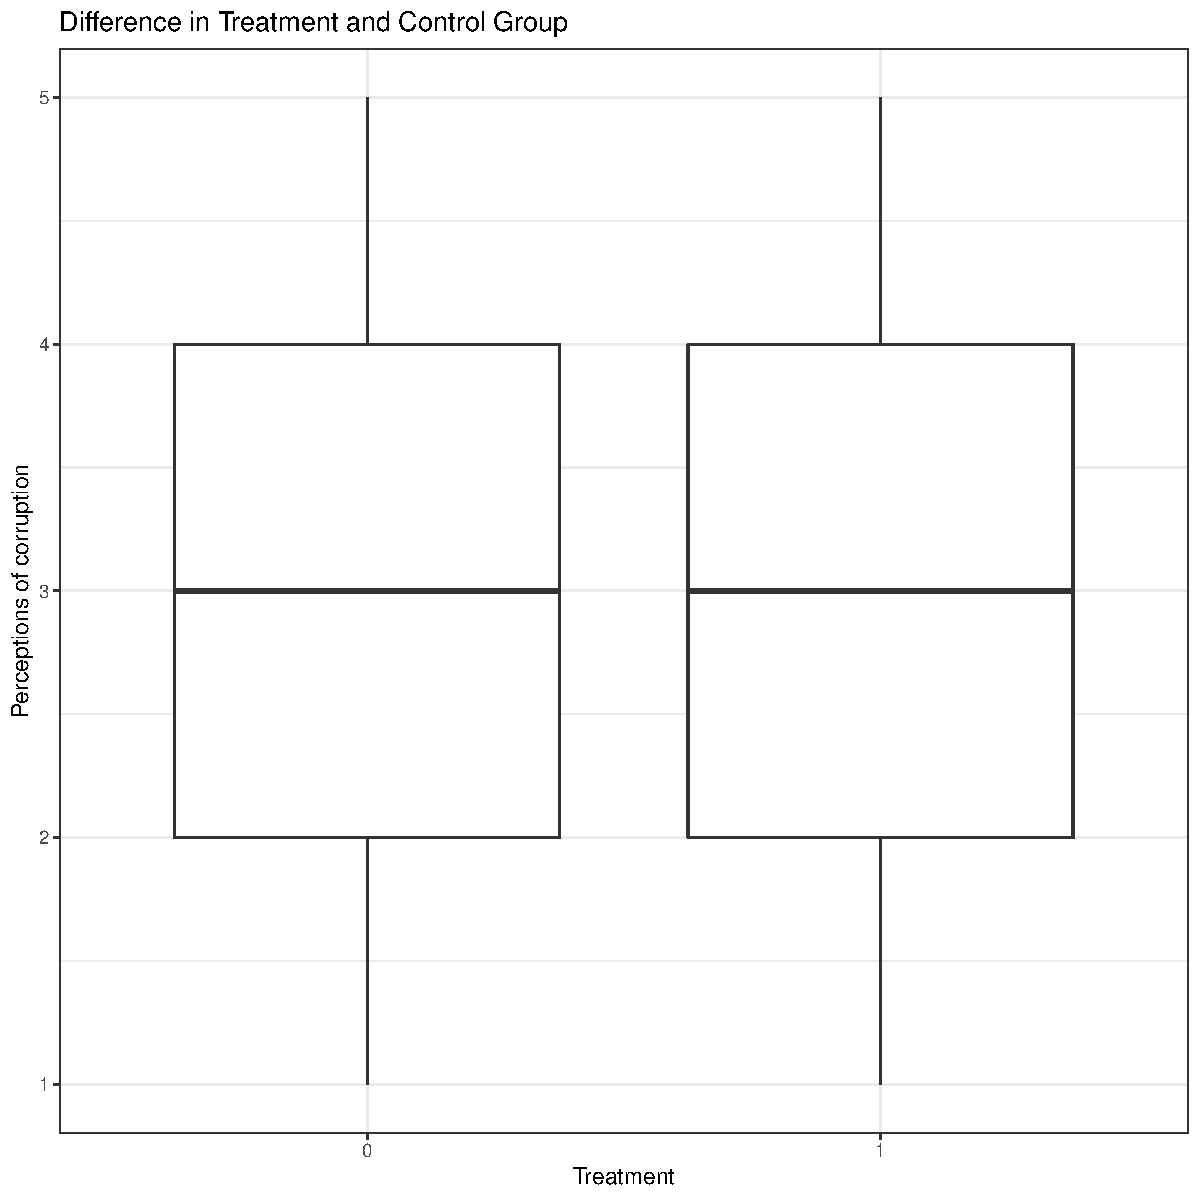
\includegraphics{PAP_Yea-Jin-Rha_files/figure-latex/mockfigure-1.pdf}

~~~~~~If the real outcome were as, I have simulated it, then the
following figure of box plot would mean that the treatment effect is
null both in the potential outcome and in the variance of the outcome.
Therefore, the empirical evidence of my study is not consistent with the
contingent self-commitment theory. They theory claims that the awareness
of corruption punishment information would induce citizen to voluntarily
engage in monitoring corruption and reduce the level of corruption
perceptions in the future. However, the null effect of the treatment in
the boxplot does not support the theoretical account.

\textbf{Appendix}

\begin{Shaded}
\begin{Highlighting}[]
\FunctionTok{library}\NormalTok{(devtools)}
\NormalTok{devtools}\SpecialCharTok{::}\FunctionTok{install\_github}\NormalTok{(}\StringTok{"viking/r{-}yaml"}\NormalTok{)}
\FunctionTok{library}\NormalTok{(RItools)}
\FunctionTok{library}\NormalTok{(xtable)}
\FunctionTok{library}\NormalTok{(DeclareDesign)}
\FunctionTok{library}\NormalTok{(ggplot2)}
\FunctionTok{library}\NormalTok{(pillar)}
\FunctionTok{library}\NormalTok{(knitr)}
\FunctionTok{library}\NormalTok{(dplyr)}

\FunctionTok{xtable}\NormalTok{(}\FunctionTok{summary}\NormalTok{(}\FunctionTok{lm\_robust}\NormalTok{(fakeC}\SpecialCharTok{\textasciitilde{}}\NormalTok{treatment, }\AttributeTok{data=}\NormalTok{ pap))}\SpecialCharTok{$}\NormalTok{coef,}\AttributeTok{label=}\StringTok{"tab:lm\_robust Regression"}\NormalTok{)}

\NormalTok{myvarest }\OtherTok{\textless{}{-}} \ControlFlowTok{function}\NormalTok{(data)\{}
\NormalTok{variance\_diff }\OtherTok{\textless{}{-}} \FunctionTok{with}\NormalTok{(data,}\FunctionTok{var}\NormalTok{(Y[Z}\SpecialCharTok{==}\DecValTok{1}\NormalTok{]) }\SpecialCharTok{{-}} \FunctionTok{var}\NormalTok{(Y[Z}\SpecialCharTok{==}\DecValTok{0}\NormalTok{]))}
\NormalTok{df }\OtherTok{\textless{}{-}} \FunctionTok{data.frame}\NormalTok{(}\AttributeTok{estimate=}\NormalTok{variance\_diff)}
\FunctionTok{return}\NormalTok{(df)}
\NormalTok{\}  }

\NormalTok{design }\OtherTok{\textless{}{-}}
  \FunctionTok{declare\_model}\NormalTok{(}\AttributeTok{data =}\NormalTok{ pap) }\SpecialCharTok{+}
  \FunctionTok{declare\_potential\_outcomes}\NormalTok{(Y}\SpecialCharTok{\textasciitilde{}}\NormalTok{ fakeC)}\SpecialCharTok{+}  \DocumentationTok{\#\#assuming true null effect}
  \FunctionTok{declare\_assignment}\NormalTok{(treatment) }\SpecialCharTok{+} 
  \FunctionTok{declare\_measurement}\NormalTok{(}\AttributeTok{Y =} \FunctionTok{reveal\_outcomes}\NormalTok{(Y }\SpecialCharTok{\textasciitilde{}}\NormalTok{ Z)) }\SpecialCharTok{+}
  \FunctionTok{declare\_inquiry}\NormalTok{(}\AttributeTok{ATE=}\FunctionTok{mean}\NormalTok{(Y\_Z\_1 }\SpecialCharTok{{-}}\NormalTok{ Y\_Z\_0))}\SpecialCharTok{+}
  \FunctionTok{declare\_inquiry}\NormalTok{(}\AttributeTok{VATE=}\FunctionTok{var}\NormalTok{(Y\_Z\_1) }\SpecialCharTok{{-}} \FunctionTok{var}\NormalTok{(Y\_Z\_0))}\SpecialCharTok{+}
  \FunctionTok{declare\_estimator}\NormalTok{(Y }\SpecialCharTok{\textasciitilde{}}\NormalTok{ Z , }\AttributeTok{model =}\NormalTok{ lm\_robust, }\AttributeTok{label =} \StringTok{"ITT"}\NormalTok{, }\AttributeTok{inquiry=}\StringTok{"ATE"}\NormalTok{)}\SpecialCharTok{+}
  \FunctionTok{declare\_estimator}\NormalTok{(}\AttributeTok{label =} \StringTok{"varest"}\NormalTok{, }\AttributeTok{inquiry=}\StringTok{"VATE"}\NormalTok{, }\AttributeTok{handler=}\FunctionTok{label\_estimator}\NormalTok{(myvarest)) }

\DocumentationTok{\#\#Power(= false positive rate in this case) and Coverage}
\FunctionTok{set.seed}\NormalTok{(}\DecValTok{123456}\NormalTok{)}
\NormalTok{diag}\OtherTok{\textless{}{-}} \FunctionTok{diagnose\_design}\NormalTok{(design, }\AttributeTok{sims =} \DecValTok{1000}\NormalTok{)}

\DocumentationTok{\#\#false positive rate}
\FunctionTok{set.seed}\NormalTok{(}\DecValTok{789789}\NormalTok{)}
\NormalTok{sim}\OtherTok{\textless{}{-}} \FunctionTok{simulate\_design}\NormalTok{(design, }\AttributeTok{sims =} \DecValTok{1000}\NormalTok{)}
\NormalTok{fpr1}\OtherTok{\textless{}{-}} \FunctionTok{mean}\NormalTok{(sim}\SpecialCharTok{$}\NormalTok{p.value[sim}\SpecialCharTok{$}\NormalTok{estimator\_label}\SpecialCharTok{==}\StringTok{"ITT"}\NormalTok{]}\SpecialCharTok{\textless{}}\FloatTok{0.1}\NormalTok{) }\DocumentationTok{\#\#alpha=0.1}
\NormalTok{fpr2}\OtherTok{\textless{}{-}}\FunctionTok{mean}\NormalTok{(sim}\SpecialCharTok{$}\NormalTok{p.value[sim}\SpecialCharTok{$}\NormalTok{estimator\_label}\SpecialCharTok{==}\StringTok{"ITT"}\NormalTok{]}\SpecialCharTok{\textless{}}\FloatTok{0.05}\NormalTok{)  }\DocumentationTok{\#\#alpha=0.05}
\NormalTok{fpr3}\OtherTok{\textless{}{-}} \FunctionTok{mean}\NormalTok{(sim}\SpecialCharTok{$}\NormalTok{p.value[sim}\SpecialCharTok{$}\NormalTok{estimator\_label}\SpecialCharTok{==}\StringTok{"ITT"}\NormalTok{]}\SpecialCharTok{\textless{}}\FloatTok{0.01}\NormalTok{)  }\DocumentationTok{\#\#alpha=0.01}
\DocumentationTok{\#\#fpr1}
\NormalTok{fpr2 }
\DocumentationTok{\#\#fpr3}
\DocumentationTok{\#\#power (assuming true effect not null)}

\NormalTok{design2  }\OtherTok{\textless{}{-}}
  \FunctionTok{declare\_model}\NormalTok{(}\AttributeTok{data =}\NormalTok{ pap) }\SpecialCharTok{+}
  \FunctionTok{declare\_potential\_outcomes}\NormalTok{(Y}\SpecialCharTok{\textasciitilde{}}\NormalTok{ fakeC}\SpecialCharTok{+}\NormalTok{ (}\SpecialCharTok{{-}}\DecValTok{1}\NormalTok{)}\SpecialCharTok{*}\NormalTok{Z)}\SpecialCharTok{+}
  \FunctionTok{declare\_assignment}\NormalTok{(treatment) }\SpecialCharTok{+} 
  \FunctionTok{declare\_measurement}\NormalTok{(}\AttributeTok{Y =} \FunctionTok{reveal\_outcomes}\NormalTok{(Y }\SpecialCharTok{\textasciitilde{}}\NormalTok{ Z)) }\SpecialCharTok{+}
  \FunctionTok{declare\_inquiry}\NormalTok{(}\AttributeTok{ATE=}\FunctionTok{mean}\NormalTok{(Y\_Z\_1 }\SpecialCharTok{{-}}\NormalTok{ Y\_Z\_0))}\SpecialCharTok{+}
  \FunctionTok{declare\_inquiry}\NormalTok{(}\AttributeTok{VATE=}\FunctionTok{var}\NormalTok{(Y\_Z\_1) }\SpecialCharTok{{-}} \FunctionTok{var}\NormalTok{(Y\_Z\_0))}\SpecialCharTok{+}
  \FunctionTok{declare\_estimator}\NormalTok{(Y }\SpecialCharTok{\textasciitilde{}}\NormalTok{ Z , }\AttributeTok{model =}\NormalTok{ lm\_robust, }\AttributeTok{label =} \StringTok{"ITT"}\NormalTok{, }\AttributeTok{inquiry=}\StringTok{"ATE"}\NormalTok{)}\SpecialCharTok{+}
  \FunctionTok{declare\_estimator}\NormalTok{(}\AttributeTok{label =} \StringTok{"varest"}\NormalTok{, }\AttributeTok{inquiry=}\StringTok{"VATE"}\NormalTok{, }\AttributeTok{handler=}\FunctionTok{label\_estimator}\NormalTok{(myvarest)) }

\FunctionTok{set.seed}\NormalTok{(}\DecValTok{1234567}\NormalTok{)}
\NormalTok{diag2}\OtherTok{\textless{}{-}} \FunctionTok{diagnose\_design}\NormalTok{(design2, }\AttributeTok{sims =} \DecValTok{1000}\NormalTok{)}
\NormalTok{diag2}

\FunctionTok{set.seed}\NormalTok{(}\DecValTok{1234567}\NormalTok{)}
\NormalTok{diag2}\OtherTok{\textless{}{-}} \FunctionTok{diagnose\_design}\NormalTok{(design2, }\AttributeTok{sims =} \DecValTok{1000}\NormalTok{)}
\FunctionTok{xtable}\NormalTok{(}\FunctionTok{summary}\NormalTok{(diag2),}\AttributeTok{label=}\StringTok{"tab:TrueEffect Diag"}\NormalTok{)}


\FunctionTok{glimpse}\NormalTok{(pap)}

\NormalTok{Y}\OtherTok{\textless{}{-}}\NormalTok{pap}\SpecialCharTok{$}\NormalTok{fakeC}
\NormalTok{df}\OtherTok{\textless{}{-}}\FunctionTok{data.frame}\NormalTok{(}
  \AttributeTok{Z=}\FunctionTok{as.character}\NormalTok{(pap}\SpecialCharTok{$}\NormalTok{treatment),}
  \AttributeTok{y0=} \FunctionTok{min}\NormalTok{(Y),}
  \AttributeTok{y25=}\FunctionTok{quantile}\NormalTok{(Y,}\FloatTok{0.25}\NormalTok{),}
  \AttributeTok{y50=} \FunctionTok{quantile}\NormalTok{(Y, }\FloatTok{0.5}\NormalTok{),}
  \AttributeTok{y75=} \FunctionTok{quantile}\NormalTok{(Y, }\FloatTok{0.75}\NormalTok{),}
  \AttributeTok{y100=} \FunctionTok{max}\NormalTok{(Y)}
  
\NormalTok{)}

\NormalTok{Boxplot}\OtherTok{\textless{}{-}}\FunctionTok{ggplot}\NormalTok{(df, }\FunctionTok{aes}\NormalTok{(Z,Y)) }\SpecialCharTok{+} 
  \FunctionTok{geom\_boxplot}\NormalTok{(}\FunctionTok{aes}\NormalTok{(}\AttributeTok{ymin=}\NormalTok{y0, }\AttributeTok{lower=}\NormalTok{y25, }\AttributeTok{middle=}\NormalTok{ y50, }\AttributeTok{upper=}\NormalTok{ y75, }\AttributeTok{ymax=}\NormalTok{ y100, }\AttributeTok{stat=}\StringTok{"identity"}\NormalTok{))}\SpecialCharTok{+}
  \FunctionTok{labs}\NormalTok{(}\AttributeTok{x=} \StringTok{"Treatment"}\NormalTok{, }\AttributeTok{y=} \StringTok{"Perceptions of corruption"}\NormalTok{, }\AttributeTok{title=}\StringTok{"Difference in Treatment and Control Group"}\NormalTok{)}\SpecialCharTok{+}
  \FunctionTok{theme\_bw}\NormalTok{()}

\DocumentationTok{\#\#another approach}
\NormalTok{Jitter}\OtherTok{\textless{}{-}} \FunctionTok{ggplot}\NormalTok{(df, }\FunctionTok{aes}\NormalTok{(Z, Y))}\SpecialCharTok{+}
  \FunctionTok{geom\_point}\NormalTok{(}\AttributeTok{position=}\StringTok{"jitter"}\NormalTok{)}
\CommentTok{\#Jitter}

\NormalTok{Boxplot}

\NormalTok{balcheck}\OtherTok{\textless{}{-}}\FunctionTok{xBalance}\NormalTok{(treatment}\SpecialCharTok{\textasciitilde{}}\NormalTok{sex }\SpecialCharTok{+}\NormalTok{ age\_quart }\SpecialCharTok{+}\NormalTok{ residence }\SpecialCharTok{+}\NormalTok{ party\_affiliation }\SpecialCharTok{+}\NormalTok{ pol\_ideo }\SpecialCharTok{+}\NormalTok{ edu }\SpecialCharTok{+}\NormalTok{ income, }\AttributeTok{data=}\NormalTok{pap, }\AttributeTok{report=}\FunctionTok{c}\NormalTok{(}\StringTok{"all"}\NormalTok{))}
\FunctionTok{xtable}\NormalTok{(}\FunctionTok{summary}\NormalTok{(}\FunctionTok{lm\_robust}\NormalTok{(fakeC}\SpecialCharTok{\textasciitilde{}}\NormalTok{treatment, }\AttributeTok{data=}\NormalTok{ pap))}\SpecialCharTok{$}\NormalTok{coef,}\AttributeTok{label=}\StringTok{"tab:lm\_robust Regression"}\NormalTok{)}
\FunctionTok{kable}\NormalTok{(}\FunctionTok{summary}\NormalTok{(diag)[, }\FunctionTok{c}\NormalTok{(}\DecValTok{2}\SpecialCharTok{:}\DecValTok{3}\NormalTok{, }\DecValTok{6}\SpecialCharTok{:}\DecValTok{14}\NormalTok{)])}

\FunctionTok{kable}\NormalTok{(}\FunctionTok{summary}\NormalTok{(diag2)[, }\FunctionTok{c}\NormalTok{(}\DecValTok{2}\SpecialCharTok{:}\DecValTok{3}\NormalTok{, }\DecValTok{6}\SpecialCharTok{:}\DecValTok{14}\NormalTok{)])}
\end{Highlighting}
\end{Shaded}

\textbf{github link} \url{https://github.com/yeajinrha/PS531_PAP.git}

\printbibliography

\end{document}
